%
% average.tex -- Average
%
% (c) 2019 Prof Dr Andreas Müller, Hochschule Rapperswil
%

\begin{frame}[fragile]
\frametitle{Averaging\uncover<6->{ --- Linearkombination von $T_k\varphi$}}

\newboolean{blocks}
\setboolean{blocks}{false}

\begin{tikzpicture}[>=latex]

	\def\punkt#1#2#3{
		2*sin(15*(#1*#3+(1-#3)*#2)*(12-(#1*#3+(1-#3)*#2)))
	}

	\def\stufe#1#2{
		\pgfmathparse{
			0.090909*(\punkt{#1}{#2}{1}+\punkt{#1}{#2}{0.1}+\punkt{#1}{#2}{0.2}+\punkt{#1}{#2}{0.3}+\punkt{#1}{#2}{0.4}+\punkt{#1}{#2}{0.5}+\punkt{#1}{#2}{0.6}+\punkt{#1}{#2}{0.7}+\punkt{#1}{#2}{0.8}+\punkt{#1}{#2}{0.9}+\punkt{#1}{#2}{0})
		}
		\xdef\y{\pgfmathresult}
		\ifthenelse{\boolean{blocks}}{
			\draw[color=red,line width=0.1pt] (#1,0)--(#1,\y);
			\draw[color=red,line width=0.1pt] (#2,0)--(#2,\y);
			\fill[color=red!10] (#1,0)--(#2,0)--(#2,\y)--(#1,\y)
				--cycle;
		}{
			\draw[color=red,line width=0.1pt] (#1,\yold)--(#1,\y);
		}
		\draw[color=red,line width=1pt] (#1,\y)--(#2,\y);
		\xdef\xold{#2}
		\xdef\yold{\y}
	}
	\def\kurve#1#2#3{
		\begin{scope}
			\clip (-0.1,-2.1) rectangle (12.3,2.1);
			\def\xold{0}
			\def\yold{0}
			\foreach \x in {#1,#2,...,#3}{
				\stufe{\xold}{\x}
			}
		\end{scope}
	}

	\ifthenelse{\boolean{presentation}}{
		\only<1>{ \kurve{1}{2}{13} }
		\only<2>{ \kurve{0.5}{1}{13} }
		\only<3>{ \kurve{0.25}{0.5}{13} }
		\only<4>{ \kurve{0.125}{0.25}{13} }
		\only<5>{ \kurve{0.0625}{0.125}{13} }

		\setboolean{blocks}{true}

		\only<6>{ \kurve{1}{2}{13} }
		\only<7>{ \kurve{0.5}{1}{13} }
		\only<8>{ \kurve{0.25}{0.5}{13} }
		\only<9>{ \kurve{0.125}{0.25}{13} }
		\only<10>{ \kurve{0.0625}{0.125}{13} }
	}{
		\kurve{0.25}{0.5}{13}
	}

	\draw[->,line width=0.7pt] (-0.1,0)--(12.6,0)
		coordinate[label={$t$}];
	\draw[->,line width=0.7pt] (0,-2.1)--(0,2.3)
		coordinate[label={right:$f$}];

	\draw[color=blue,line width=1pt] plot[domain=0:12.2,samples=1000]
		({\x},{2*sin(15*\x*(12-\x))});

\end{tikzpicture}

\end{frame}





